\documentclass[8pt,landscape]{article}
\usepackage[a4paper,top=0.5cm,bottom=0.5cm,left=0.5cm,right=0.5cm]{geometry}

\usepackage[ngerman]{babel}
\usepackage{graphicx}
\usepackage[utf8]{inputenc}
\usepackage{amsfonts}
\usepackage{multicol}
\setlength\parindent{0ex}
\usepackage{amsmath}
\setlength{\columnsep}{10mm}
\usepackage{blindtext}
\usepackage{paralist}
\usepackage{bbm} % Natural numbers etc.

% Use compactitem.



% -------------- Beginning of Document ---------------.
\begin{document}


\renewcommand{\labelitemi}{--}
%\setlist{noitemsep}
\pagestyle{empty}
\raggedright
\setlength{\columnsep}{2mm}
\setlength{\columnseprule}{0.1mm}
\begin{multicols}{3}
\title{\textbf{Autonomous Mobile Robots}}
\author{Fabian Blöchliger}
\date{Spring Semester 2016}
\maketitle


\section{Introduction and Motivation}

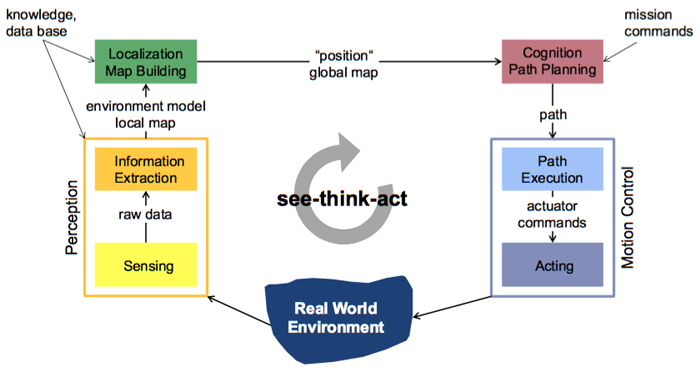
\includegraphics[width=\columnwidth]{img/1_SeeThinkAct.png}

\section{Locomotion Concepts}

To get from the inertial frame $I$ to body frame $B$:
\begin{compactitem}
\item \textbf{translate} with vector ${}_I\mathbf{r}_{OB}$,
\item \textbf{rotate} with matrix $\mathbf{R}_{IB}$.
\end{compactitem}

\vspace{5pt}

Express point $P$ which is given w.r.t frame $B$ in frame $I$:

\vspace{-5pt}
\begin{center}
${}_I\mathbf{r}_{OP} = {}_I\mathbf{r}_{OB} +
\mathbf{R}_{IB}\;{}_B\mathbf{r}_{BP}$.
\end{center}

Equivalent \textbf{homogeneous transformation} description:

\vspace{-5pt}
\begin{center}
  $\left(\begin{matrix}
    {}_I\mathbf{r}_{OP} \\
    1
  \end{matrix}\right)
  =
  \left(\begin{matrix}
    \mathbf{R}_{IB} & {}_I\mathbf{r}_{OB} \\
    0 & 1
  \end{matrix}\right)
  \left(\begin{matrix}
    {}_B\mathbf{r}_{BP} \\
    1
  \end{matrix}\right)$
\end{center}

Basic rotation matrices $\mathbf R_x(\bullet)$, $\mathbf R_y(\bullet)$, $\mathbf
R_z(\bullet)$:

\vspace{-5pt}
\begin{center}
  $\left(\begin{matrix}
    1 & 0 & 0 \\
    0 & \cos & -\sin \\
    0 & \sin & \cos
  \end{matrix}\right),\;
  \left(\begin{matrix}
    \cos & 0 & \sin \\
    0 & 1 & 0 \\
    -\sin & 0 & \cos
  \end{matrix}\right),\;
  \left(\begin{matrix}
    \cos & -\sin & 0 \\
    \sin & \cos & 0 \\
    0 & 0 & 1
  \end{matrix}\right).$
\end{center}

\textbf{Jacobian} (partial derivative of position vector $\mathbf{r}_{OP}$
w.r.t. \textbf{generalized coordinate} vector $\mathbf{q}$):

\vspace{-5pt}
\begin{center}
  $J_P = \dfrac{\partial \mathbf{r}_{OP}(\mathbf q)}{\partial \mathbf q}$.
\end{center}

\section{Mobile Robot Kinematics}

\blindtext[3]

\section{Perception I}

\blindtext[3]

\section{Perception II}

\blindtext[3]

\section{Perception III}

\blindtext[3]

\section{Perception IV}

\blindtext[3]

\section{Localization I}

\blindtext[3]

\section{Localization II}

\blindtext[3]

\section{SLAM I}

\blindtext[3]

\section{SLAM II}

\blindtext[3]

\section{Planning I}

\blindtext[3]

\section{Planning II}

\blindtext[3]





\end{multicols}

% -------------- End of Document ---------------------. 
\end{document}
